\scanpage{48}

Pour le voir, on est ramené par un
dévissage facile, [utiliser l'existence d'une suite exacte
\diagram{\begin{tikzcd}[column sep=small]
0\arrow[r,dash]&P'\arrow[r,dash]&F'\arrow[r,dash]&\widetilde F'\arrow[r,dash]&Q'\arrow[r,dash]&0
\end{tikzcd}}
où $\operatorname{supp}P'\subset Y'$, $\operatorname{supp}Q'\subset Y'$,
$\dim\operatorname{supp}P'\leq0$, $\dim\operatorname{supp}Q'\leq1$,
et $\operatorname{prof}\unsure{\hat F'_{x'}|\widetilde F'_{x'}}$
\unsure{aux} $\forall$ pts fermés de $X'$ -- pas seulement de
$X'-Y'$] -- dévissage qui est une question purement locale
sur le schéma de \uline{Jacobson} $X'$] au cas où on a
$\operatorname{prof}F_x\ge2$, \deleted{D'ailleurs, si}
pour \uline{$\forall$ $x\in X'$}. Soit
d'ailleurs $K'$ le noyau de la multiplication par
\deleted{\unsure{sur $F_x$}}
$t^n$ ($n$ grand) on a
\diagram{\begin{tikzcd}[column sep=small]
0\arrow[r,dash]&K'\arrow[r,dash]&F'\arrow[r,dash]&C'\arrow[r,dash]&0
\end{tikzcd}}
\deleted{avec $C'$} $t$ \deleted{est} $C'$-régulier. On a

\margin{\figure{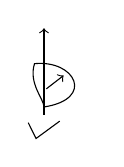
\begin{tikzpicture}[x=1cm,y=1cm]
\draw[->] (0,0)--(0,1.1);
\draw (0,.1) .. controls (.65,.2) and (.4,.7) .. (-.12,.65)
 .. controls (-.2,.4) and (0,.2) .. (0,.1);
\draw[->] (.03,.33)--(.25,.5);
\draw (-.2,-.1)--(-.1,-.3)--(.2,-.08);
\end{tikzpicture}}}

\margin{\figure{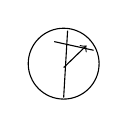
\begin{tikzpicture}[x=1cm,y=1cm]
\draw (0,0) ellipse (.45 and .45);
\draw (0,-.43)--(.05,.42);
\draw (-.12,.28)--(.38,.17);
\draw[->] (0,-.05)--(.29,.23);
\end{tikzpicture}}}

\diagram{\begin{tikzcd}[column sep=small,row sep=large]
&0\arrow[r,dash]&\Gamma K'\arrow[r]\arrow[d,"\sim"']&
\Gamma F'\arrow[r,dash]\arrow[d]&\Gamma C'\arrow[r,dash]\arrow[d,"\sim?"']&
H^1\unsure{K'|C'}\arrow[d,phantom,"\rotatebox{90}{$\simeq$}"]\\
A\quad\unsure{\hat A_\Phi|\hat A_\varphi}&0\arrow[r,dash]&\Gamma\hat K'\arrow[r,dash]&
\Gamma\hat F'\arrow[r,dash]&\Gamma\unsure{\hat C'|\hat G'}\arrow[r,dash]&H^1\unsure{\hat K'|\hat C'}
\end{tikzcd}}

On est ramené au cas où $t$ est \unsure{non} div. de $0$.

\figure{
\begin{tikzpicture}\draw (0,0)--(12,.3);\end{tikzpicture}}

\margin{47}
